\subsubsection{Overview \cite{LHeC:Birmingham}}

The LHeC has been proposed as a colliding beam facility at CERN. It will exploit the high energies already available at the LHC for lepton-nucleon collisions. An existing LHC proton or heavy ion beam will be used to collide with a new, high energy, electron beam; this will occur simultaneously with the LHC’s current proton-proton experiments.
 
In the current design (figure 1), the electron beam is accelerated passing multiple times through a pair of linear accelerators in a racetrack configuration, producing an energy of 60 GeV at the interaction point. This results in an unprecedented kinematic range for lepton-nucleon scattering: the centre of mass energy will be 1.3 TeV The luminosity of $10^{33}$ \textemdash $10^{34} cm^{-2}s^{-1}$ is two orders of magnitude larger than previous similar proposals.

\begin{figure}[!htb]
\centering
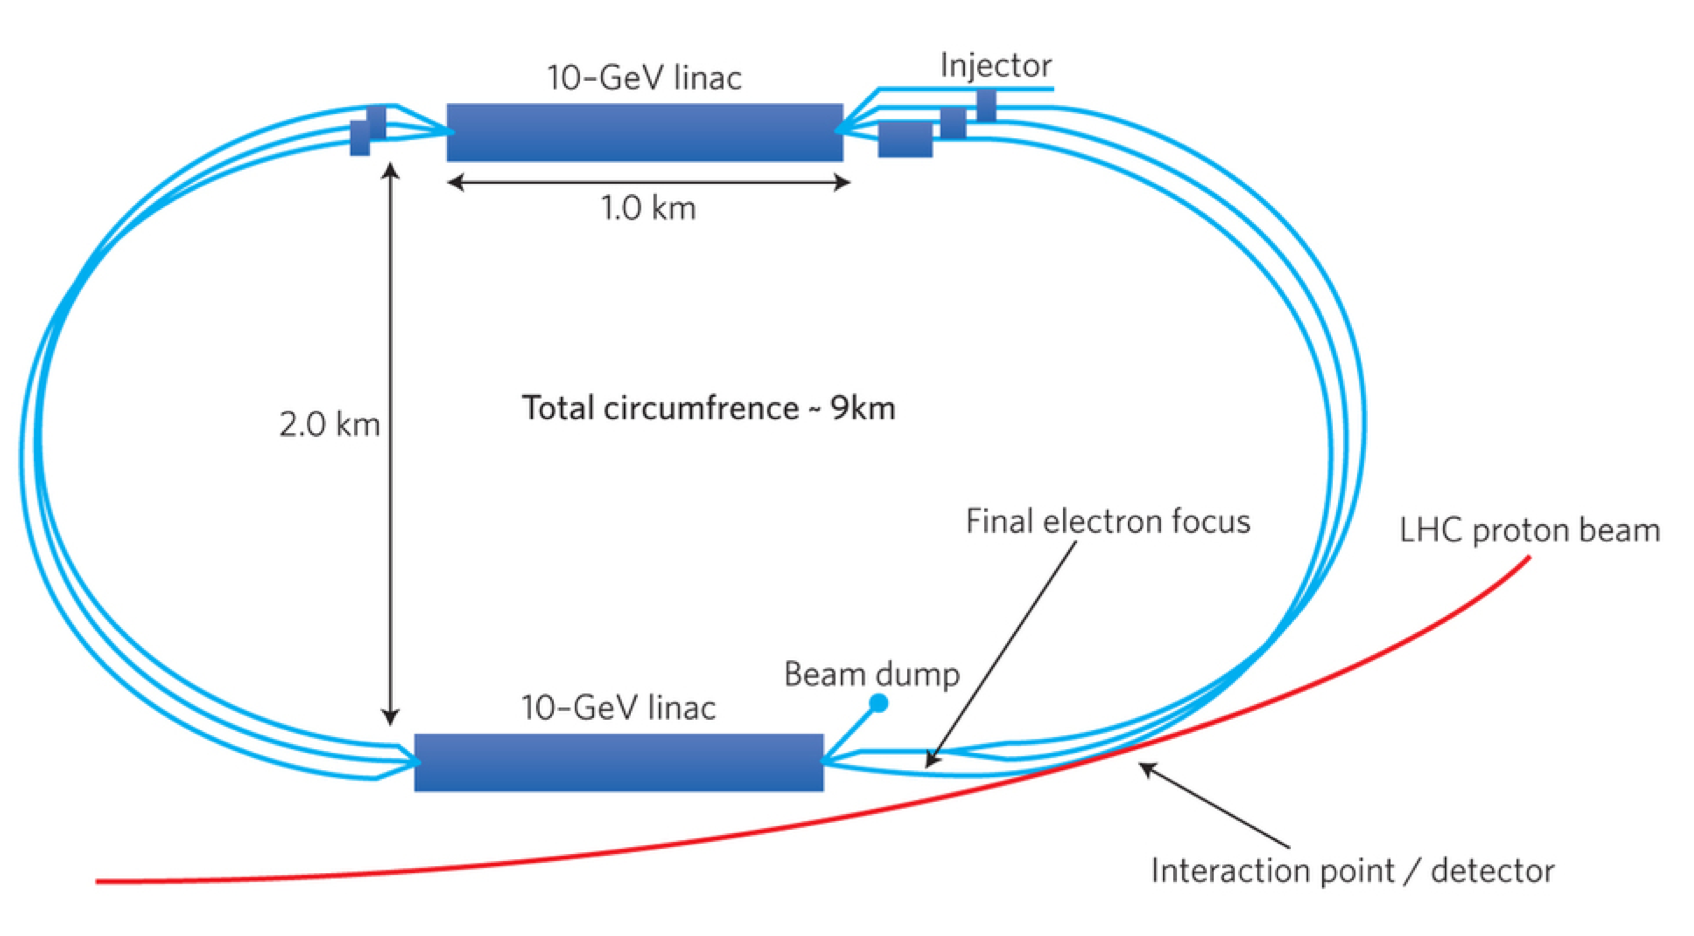
\includegraphics[width=0.9\textwidth]{LHeC_Diagram.png}
\caption{The current layout of the proposed electron ring (blue) next the a section of the LHC’s proton accelerating ring (red).
}
\end{figure}

\subsubsection{Goals}

The goals of the LHeC are as follows:
\begin{itemize}
\item Explore quantum chromo dynamics in greater detail with greater precision.
\item Examine the strong nuclear interaction in greater detail with greater precision.
\item Potentially use it as a rich source of the Higgs Boson and thus explore its interaction strength, mass and spin.
\item Able to produce Charm, Top and Bottom quarks for greater examination.
\end{itemize}
As the collider will use electron-proton collisions it will make it an invaluable tool in the examination of the structure of the proton, as it will provide cleaner reactions than are currently possible at the LHC.
 
\subsubsection{Feasibility}

The proton side of the design will incorporate the already functional proton accelerator that is built at the LHC and thus there will be no feasibility issues with this. On top of this the current LHC experiments can continue to run during the construction of the collider and will continue to be run once it is operational, there is a small risk of interruption during the tunnel excavation phase due to the proximity to the LHC ring. This then means that the LHC will continue to push the energy boundaries whilst the LHeC can examine the structure of the proton and the Higgs boson in greater detail. Also if any new discoveries are made in the energy scale of 1.3TeV at the LHC it will be possible to test them with greater precision using the LHeC.
 
The electron beam will not use any new technologies in its creation; the only issue that will arise is attempting to match its circumference to that of the proton ring. Though civil engineers have already considered this and have declared it feasible. \cite{LHeC:Report}
 
Overall the design is feasible, and this will not be a problem is implementing the construction of the LHeC.
 
\subsubsection{Spin Offs}

There are few unique spin offs relevant to this collider, as its goal is to probe the structure of the proton with more precision it is entirely possible that spin offs will emerge after its construction that may result from this greater understanding.
 
The main, somewhat generic, spin off is the improvement of data transfer in computing. This will allow communication to occur at much greater rates between computers and allow much larger arrays of data to be generated faster.
 
A more unique spin off is the improvement of viability of PET due to SCRFs. Superconducting Radiofrequency acceleration is the production of high quality and energy X-Rays using Inverse Compton Scattering (ICS). ICS is the transfer of energy from an electron to a photon. ICS only exists in nature at the accretion disk of a black hole, where slow photons are collided with fast electrons causing X-Ray spectra. However it may be possible to generate these frequencies colliding a fast proton and electron at LHeC.
 
\subsubsection{Cost}

Detailed cost analyses have yet to be produced, as the project has not gained much momentum in the physics community. One estimate put the cost at $\sim$\$50M \cite{LHeC:Zimmermann}. This costing seems very low and may fail to take into account any of the cost considerations involved in digging the tunnels. Though because a large part of the design incorporates the already functional LHC the costs would be lower than other proposed colliders.
 
 
\subsubsection{Time scale}

As all of the technology required is already in production and used in modern colliders there would be very little (possibly no) research and development time needed before construction could begin.
 
The total estimated time; from starting the assembly of the main detector elements on the surface to the commissioning of the detector underground is 30 months. The field map would take one extra month.
 
\subsubsection{Conclusion}

Though the design is feasible, the costs potentially low and the time scale short; construction of this collider is not recommended. This is because the physics that this collider could explore is not nearly as interesting as that proposed by other colliders. The structure of the proton may be further explored in higher energy experiments at CERN’s LHC and the commission of a new facility to explore this is unnecessary. Finally other proposed colliders provide a much cleaner and precise process to look at the mass, interaction strength and spin of the Higgs particle.